\documentclass[margin=10pt]{standalone}
\usepackage{pgfplots}
\pgfplotsset{compat=1.8}
\usepackage{lmodern}

\tikzset{
	every pin/.style={
		font=\scriptsize,
		pin distance=4ex},
	small dot/.style={
		fill=gray,
		circle,
		scale=0.1}
}

\begin{document}
	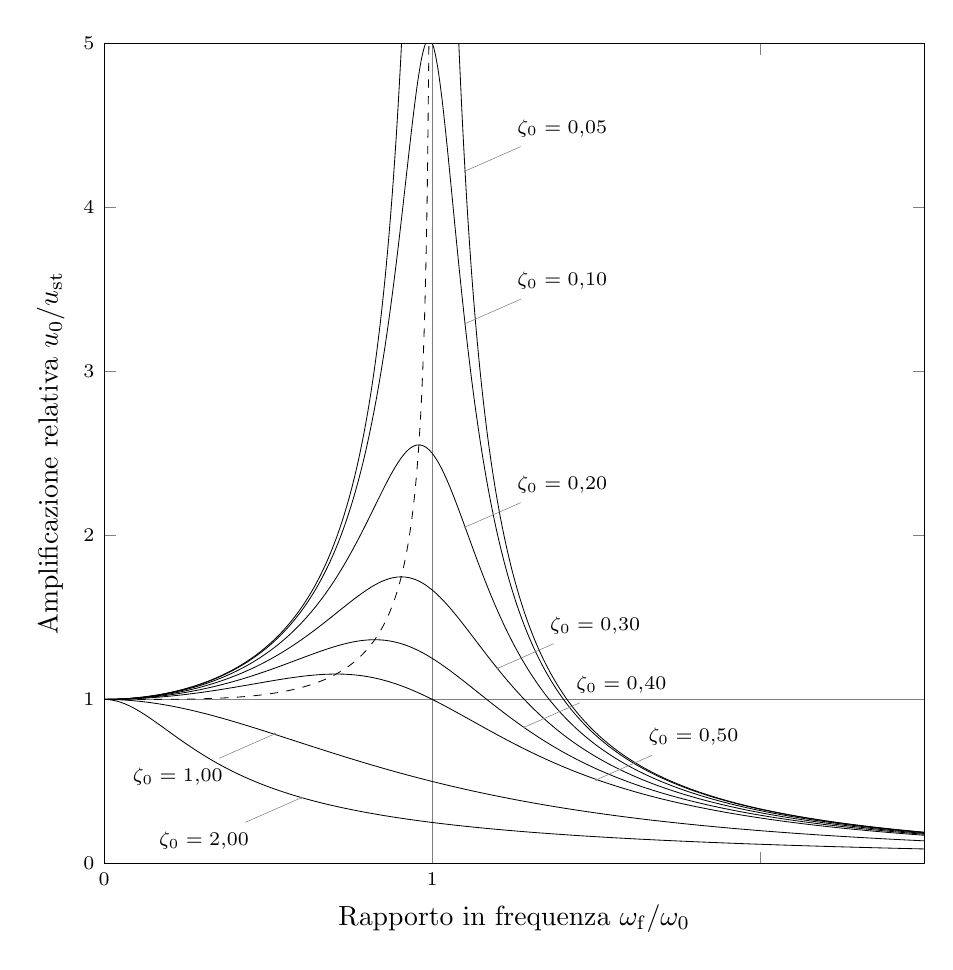
\begin{tikzpicture}
	\begin{axis}[
	% labels
	tick label style={font=\scriptsize},
	xlabel={Rapporto in frequenza $\omega_\mathrm{f}/\omega_0$},
	ylabel={Amplificazione relativa $u_0/u_\mathrm{st}$},
	ytick={0,1,2,3,4,5},
	xtick={0,1,2,3},
	xticklabels={0,1,,},
	%
	% plot lines property
	no markers,
	line width=0.3pt,
	cycle list={{black,solid}},
	%
	% dominio 2D
	samples=200,
	smooth,
	domain=0:2.5,
	xmin=0, xmax=2.5,
	ymin=0, ymax=5.0,
	%
	% canvas dimensions
	width=12cm, height=12cm
	]
	
	% horizontal help line
	\draw[help lines] (axis cs:0,1) -- (axis cs:2.5,1);
	% vertical help line
	\draw[help lines] (axis cs:1,0) -- (axis cs:1,5);
	
	% tracciamento curve
	\addplot {1/sqrt((1-x^2)^2+4*0.05^2*x^2)};
	\addplot {1/sqrt((1-x^2)^2+4*0.10^2*x^2)};
	\addplot {1/sqrt((1-x^2)^2+4*0.20^2*x^2)};
	\addplot {1/sqrt((1-x^2)^2+4*0.30^2*x^2)};
	\addplot {1/sqrt((1-x^2)^2+4*0.40^2*x^2)};
	\addplot {1/sqrt((1-x^2)^2+4*0.50^2*x^2)};
	\addplot {1/sqrt((1-x^2)^2+4*1.00^2*x^2)};
	\addplot {1/sqrt((1-x^2)^2+4*2.00^2*x^2)};
	
	% tracciamento funzione dei massimi
	\addplot[dashed,domain=0:0.99] {1/sqrt(1-x^4)};
	
	% etichette curve
	\node[small dot,pin=30:{$\zeta_0=0{,}05$}] at
	(axis cs:1.10,4.22) {};
	\node[small dot,pin=30:{$\zeta_0=0{,}10$}] at
	(axis cs:1.10,3.29) {};
	\node[small dot,pin=30:{$\zeta_0=0{,}20$}] at
	(axis cs:1.10,2.05) {};
	\node[small dot,pin=30:{$\zeta_0=0{,}30$}] at
	(axis cs:1.20,1.19) {};
	\node[small dot,pin=30:{$\zeta_0=0{,}40$}] at
	(axis cs:1.28,0.83) {};
	\node[small dot,pin=30:{$\zeta_0=0{,}50$}] at
	(axis cs:1.50,0.51) {};
	
	\node[small dot,pin=210:{$\zeta_0=1{,}00$}] at
	(axis cs:0.52,0.79) {};
	\node[small dot,pin=210:{$\zeta_0=2{,}00$}] at
	(axis cs:0.60,0.40) {};
	\end{axis}
	\end{tikzpicture}
\end{document}